\chapter{Background}

\section{Cryptocurrencies}
Before going delving into the financial side of the project, it is important to understand the underlying assets and the technology that drive them.

\subsection{Blockchain}
The building blocks of cryptocurrencies comes from blockchain. Blockchain is a distributed ledger that stores data, in blocks, in a chain, comprising the data itself as well has a full transaction history \cite{nofer2017blockchain}. Below shows a diagram of blocks in a blockchain.

\begin{figure}[!htb]
    \centering
    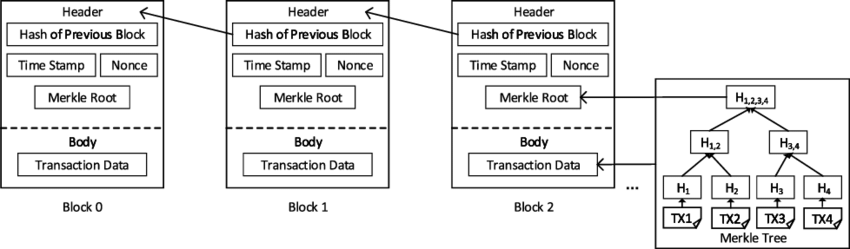
\includegraphics[width=0.8\textwidth]{background/Images/The-structure-of-a-Blockchain.png}
    \caption{Blockchain Diagram \cite{inbookBlockchain}}
\end{figure}

\subsubsection{Header, Hash of Previous Block and Timestamp}
The timestamp and hashes of the block and its' predecessing block are all used to ensure the ordering of blocks within a chain. By hashing the data to a fixed size, and storing in its succeeding block makes the tampering of chains difficult as it would mean the chain deviates from its old state. In addition to this, by hashing and using Nonce, blockchain employs the Proof-of-Work algorithm to ensure correctness. The Proof-of-Work algorithm is used to confirm and add new transaction to the chain.

\subsubsection{Nonce}
A nonce, `Number Only used Once', is a number that is added to a hashed block to make the transaction more secure. It is randomly generated which miners use to validate a transaction. A miner first guesses a nonce, appends the guess to the hash of the current header. The miner then rehashes the value and compares this to the target hash. If the guess was correct, the miner is granted the block \cite{noauthor_components_2021}. 

\subsubsection{Merkle root}
A merkle root is also stored in each block to validate transactions in an efficient manner, in terms of storage and searching. A merkle tree is a a tree of hashes where each leaf node is it's data hash and it's parent node, the hash of their children's hashes. In storing the merkle root, we do not need to directly store each transaction in each block, and also allows a quick search for any malicious alterations in differing blocks\cite{noauthor_merkle_nodate}.

\subsection{Decentralised Finance}
One of the first application of blockchain was by Satoshi Nakamoto to create the first `purely peer-to-peer version of electronic cash' \cite{nakamoto2009bitcoin}. Nakamoto's solution details the process in which a decentralised, peer to peer approach to verify and track transactions without a centralized institution.

\subsection{Exchanges}

\section{Arbitrage}
Arbitrage is the process in which a trader simultaneously buys and sells an asset in order to take advantage of a market inefficiency \cite{businessinsightsblog_2021}. Arbitrage is also possible in other types of securities by finding price inefficiencies in the prices of options, forward contracts and other exotics.


Sources have shown that the word ``\textit{Arbitrage}'' has been used as early as the Renaissance era wehere surviving documents showed a large amount of bills being exchanged \cite{poitras_2021}. There has also been some evidence to suggest that arbitrage was used as early as the Greek and Roman eras. Objects such as Sumerian cuneiform tablets show trade of ancient bills however we cannot come to strong conclusions of this. Early forms of arbitrage would likely to have been purchasing a commodity then transporting them to a foreign land and selling them at a higher price. This is type of arbitrage is called commodity arbitrage and is still is applicable today. With the example above, transporting the goods takes a significant amount of to the merchant, trader, which could cause variations in the price, however in the modern day this has been reduced and with electronic exchanges this time to buy and sell is very small. This means inefficiencies in the market, where a trader can profit purely by buying and selling, should not exist. This is called the ``Law of One Price''. The ``Law of One Price'' states that every identical commidty or asset should have the same price regardless of exchange or location, given there are no transaction costs, no transportation costs, no legal restrictions, the exchange rates are the same and no market manipulation occurs \cite{noauthor_law_nodate}. This is because if this were not the case, an arbitrage opportunity would arise and someone would take advantage of the scenario causing the prices on both markets to converge due to the market forces. In the real world arbitrage opportunities are tremendously common, thus allowing a risk-free investment \cite{10.2307/1828075, RICHARDSON1978341}. This project shows how these opportunities can be exploited both in a pure manner as well as using statistical methods.

\section{State of Art}
\subsection{Pure Arbitrage Techniques}
\subsection{Statistical Arbitrage Techniques}

\begin{enumerate}
    \item \cite{PAUNACristian2018ATSf} - % http://revistaie.ase.ro/content/86/04%20-%20pauna.pdf
    \item \cite{MakarovIgor2020Taai} - %https://library-search.imperial.ac.uk/permalink/44IMP_INST/fv0fdm/cdi_proquest_journals_2352592018
    \item \cite{HuangJianfeng2022Taaf} - %https://library-search.imperial.ac.uk/permalink/44IMP_INST/fv0fdm/cdi_informaworld_taylorfrancis_310_1080_13504851_2021_1930998
    \item \cite{alma991000411969901591} - %https://library-search.imperial.ac.uk/permalink/44IMP_INST/mek6kh/alma991000411969901591
    \item \cite{byrneexploration} - %https://www.scss.tcd.ie/Donal.OMahony/bfg/202021/StephenByrneDissertation.pdf
    \item \cite{6974093} - %
    \item \cite{https://doi.org/10.1111/joes.12153} - % https://onlinelibrary.wiley.com/doi/epdf/10.1111/joes.12153?saml_referrer
    \item \cite{KRAUSS2017689} - % https://www.sciencedirect.com/science/article/pii/S0377221716308657
    \item \cite{2019} - %https://www.mdpi.com/1911-8074/12/1/31 
    \item \cite{dempsey_market_2017} - %http://www.hedempsey.com/papers/Pairs%20Trading%20with%20a%20Kalman%20Filter.pdf
    \item \cite{mo_theoretical_nodate} - %https://w4.stern.nyu.edu/finance/docs/pdfs/PhD/mo-job-market.pdf
    \item \cite{crepelliere_arbitrage_2022} - %https://papers.ssrn.com/abstract=3606053
    \item \cite{wang_cyclic_2022} - %https://arxiv.org/pdf/2105.02784v3.pdf
    \item \cite{8957853} - %https://ieeexplore.ieee.org/document/8957853
    \item \cite{8450775} - %https://ieeexplore.ieee.org/document/8450775
    \item \cite{} - %https://library-search.imperial.ac.uk/permalink/44IMP_INST/mek6kh/alma991000343762601591
    \item \cite{alma991000607977501591} - %https://library-search.imperial.ac.uk/permalink/44IMP_INST/mek6kh/alma991000607977501591
    \item \cite{} - %https://library-search.imperial.ac.uk/permalink/44IMP_INST/mek6kh/alma996037714401591
    \item \cite{} - %https://library-search.imperial.ac.uk/permalink/44IMP_INST/mek6kh/alma991000617323401591
    \item \cite{alma991000475380901591} - %https://library-search.imperial.ac.uk/permalink/44IMP_INST/mek6kh/alma991000475380901591
    \item \cite{GoncuAhmet2016SAwP} - %https://library-search.imperial.ac.uk/permalink/44IMP_INST/fv0fdm/cdi_proquest_journals_1792704856
    \item \cite{ZipingZhao2019OMPW} - %https://library-search.imperial.ac.uk/permalink/44IMP_INST/fv0fdm/cdi_proquest_journals_2180047502
    \item \cite{Figa-TalamancaGianna2021Cdff} - %https://library-search.imperial.ac.uk/permalink/44IMP_INST/fv0fdm/cdi_proquest_journals_2610095214
    \item \cite{RICHARDSON1978341} - %https://www.sciencedirect.com/science/article/pii/0022199678900272
    \item \cite{poitras_2021} - %https://www.cambridge.org/core/journals/financial-history-review/article/origins-of-arbitrage/FD1A30E926696989376EDF449F9797BF
    \item \cite{businessinsightsblog_2021} - %https://online.hbs.edu/blog/post/what-is-arbitrage
    \item \cite{10.2307/1828075} - %
    \item \cite{noauthor_law_nodate} - %https://www.investopedia.com/terms/l/law-one-price.asp
    \item \cite{nakamoto2009bitcoin} - %Nakamoto bitcoin
    \item \cite{nofer2017blockchain} - %Blockchain
    \item \cite{inbookBlockchain} - % Blockchain diagram
    \item \cite{noauthor_components_2021} - % Blockchain
    \item \cite{noauthor_merkle_nodate} - % Merkle Tree
\end{enumerate}